\chapter{Assignment}
\section{MCQ}
\begin{enumerate}
	\item One of the possible solutions of the differential equation
	$y \sqrt{\left(1+x^{2}\right)} d y+x \sqrt{\left(1+y^{2}\right)} d x=0$ (where $c$ is some constant) is
	 \begin{tasks}(2)
		\task[\textbf{a.}]$\left(\sqrt{1+y^{2}}\right)\left(\sqrt{1+x^{2}}\right)=c$
		\task[\textbf{b.}]$\frac{\sqrt{1+y^{2}}}{\sqrt{1+x^{2}}}=c$
		\task[\textbf{c.}]$\sqrt{1+y^{2}}+\sqrt{1+x^{2}}=c$
		\task[\textbf{d.}]  $\sqrt{1+y^{2}}-\sqrt{1+x^{2}}=c$
	\end{tasks}
	\item The solution of the differential equation $x \frac{d y}{d x}+\cot y=0$, subject to the initial condition $y=\frac{\pi}{4}$ at $x=\sqrt{2}$ is
	 \begin{tasks}(2)
		\task[\textbf{a.}]$x=2 \cos y$
		\task[\textbf{b.}]$x=2 \sec y$
		\task[\textbf{c.}]$x=2 \sin y$
		\task[\textbf{d.}]  $x=2 \operatorname{cosecy}$
	\end{tasks}
	\item The solutions to the differential equation $\frac{d y}{d x}=-\frac{x}{y+1}$ are a family of
	 \begin{tasks}(2)
		\task[\textbf{a.}]Circles with different radii
		\task[\textbf{b.}]Circles with different centres
		\task[\textbf{c.}]Straight lines with different slopes
		\task[\textbf{d.}] Straight lines with different intercepts on the $y$-axis
	\end{tasks}
	\item The solution of the differential equation $x y \frac{d y}{d x}=3 y^{2}+x^{2}$ with the initial condition $y=2$ when $x=1$ is
	 \begin{tasks}(2)
		\task[\textbf{a.}]$2 y^{2}+x^{2}=9 x^{6}$
		\task[\textbf{b.}] $y^{2}+2 x^{2}=9 x^{6}$
		\task[\textbf{c.}] $2 y^{2}+x^{2}=8 x^{6}$
		\task[\textbf{d.}] $y^{2}+2 x^{2}=8 x^{6}$
	\end{tasks}
	\item The solution of the differential equation
	$(x+2 y)(d x-d y)=d x+d y$ (where $a$ is some constant) is
	 \begin{tasks}(2)
		\task[\textbf{a.}]$3 x+3 y+a=2 \log (3 x+6 y-1)$
		\task[\textbf{b.}] $3 x-3 y+a=2 \log (3 x+6 y-1)$
		\task[\textbf{c.}]$3 x-3 y+a=2 \log (3 x-6 y-1)$
		\task[\textbf{d.}] $3 x+3 y+a=2 \log (3 x-6 y-1)$
	\end{tasks}
	\item For the differential equation $\frac{d y}{d x}+3 y=e^{2 x}$, the possible solution is:
	 \begin{tasks}(2)
		\task[\textbf{a.}]$y=c_{1} e^{2 x}+c_{2} e^{3 x}$
		\task[\textbf{b.}]$y=c_{1} e^{-2 x}+c_{2} e^{3 x}$
		\task[\textbf{c.}]$y=c_{1} e^{2 x}+c_{2} e^{-3 x}$
		\task[\textbf{d.}] $y=c_{1} e^{-2 x}+c_{2} e^{-3 x}$
	\end{tasks}
	\item The solution of the differential equation for $y: x \frac{d y}{d x}+y=x^{4}$, subject to the initial condition $y=1$ at $x=1$ is
	 \begin{tasks}(2)
		\task[\textbf{a.}]$y=5 x^{4}-4$
		\task[\textbf{b.}]$y=\frac{x^{4}}{5}+\frac{4 x}{5}$
		\task[\textbf{c.}] $y=\frac{x^{4}}{5}+\frac{1}{5 x}$
		\task[\textbf{d.}] $y=\frac{x^{4}}{5}+\frac{4}{5 x}$
	\end{tasks}
	\item Which one of the following curves gives the solution of the differential equation $K_{1} \frac{d x}{d t}+K_{2} x=K_{3}$, where $K_{1}, K_{2}$ and $K_{3}$ are positive constants with initial conditions $x=0$ at $t=0$ ?
	 \begin{tasks}(2)
		\task[\textbf{a.}]
		\begin{figure}[H]
			\centering
			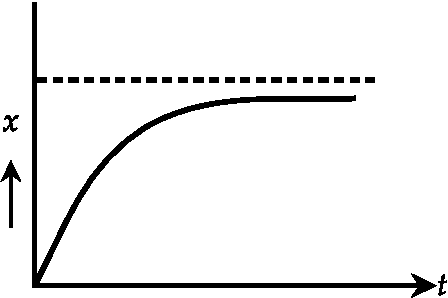
\includegraphics[height=2.5cm,width=4cm]{DE -assignment-04}
		\end{figure}
		\task[\textbf{b.}]	
		\begin{figure}[H]
			\centering
			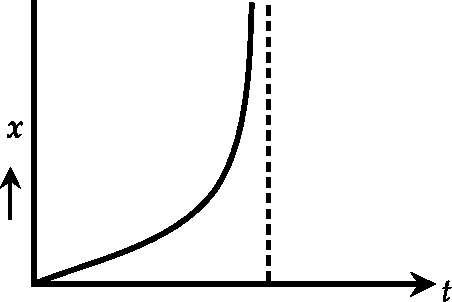
\includegraphics[height=2.5cm,width=4cm]{DE -assignment-01}
		\end{figure}
		\task[\textbf{c.}]
			\begin{figure}[H]
			\centering
			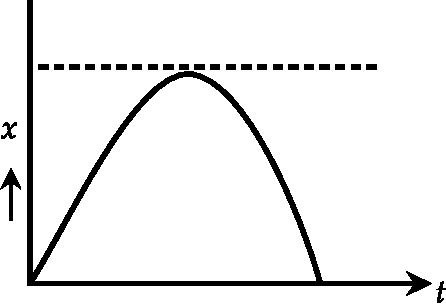
\includegraphics[height=2.5cm,width=4cm]{DE -assignment-02}
		\end{figure}
		\task[\textbf{d.}]
			\begin{figure}[H]
			\centering
			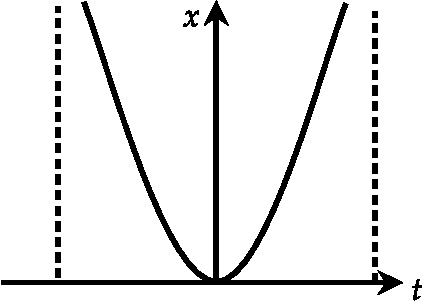
\includegraphics[height=2.5cm,width=4cm]{DE -assignment-03}
		\end{figure}
	\end{tasks}
	\item The solution of the differential equation $t \frac{d y}{d t}+y \log y=t y e^{t}$
	 \begin{tasks}(2)
		\task[\textbf{a.}]$\log y=(t+1) e^{t}+c$
		\task[\textbf{b.}]$\log y=(t-1) e^{t}+c$
		\task[\textbf{c.}]$t \log y=(t+1) e^{t}+c$
		\task[\textbf{d.}] $t \log y=(t-1) e^{t}+c$
	\end{tasks}
	\item The solution of the differential equation
	$\left(1+y^{2}\right) d x=\left(\tan ^{-1} y-x\right) d y$ (where $c$ is some constant) is
	 \begin{tasks}(2)
		\task[\textbf{a.}] $x=\left(\tan ^{-1} y+2\right)+c e^{-\tan ^{-1} y}$
		\task[\textbf{b.}] $x=\left(\tan ^{-1} y-2\right)+c e^{-\tan ^{-1} y}$
		\task[\textbf{c.}] $x=\left(\tan ^{-1} y+1\right)+c e^{-\tan ^{-1} y}$
		\task[\textbf{d.}]  $x=\left(\tan ^{-1} y-1\right)+c e^{-\tan ^{-1}y}$
	\end{tasks}
	\item The solution of the differential equation
	$y \log y \frac{d x}{d y}+x-\log y=0$ (where $c$ is some constant) is
	 \begin{tasks}(2)
		\task[\textbf{a.}]$x \log y=\frac{1}{2}(\log y)^{2}+c$
		\task[\textbf{b.}] $x \log y=2(\log y)^{2}+c$
		\task[\textbf{c.}]$x \log y=\frac{1}{2}(\log y)^{3}+c$
		\task[\textbf{d.}]  $y \log x=\frac{1}{2}(\log y)^{2}+c$
	\end{tasks}
	\item The solution of the differential equation
	$\left(e^{y}+2\right) \sin x d x-e^{y} \cos x d y=0$ (where $c$ is some constant) is
	 \begin{tasks}(2)
		\task[\textbf{a.}]$\left(e^{y}+2\right) \sin x=c$
		\task[\textbf{b.}] $\left(e^{y}+2\right) \cos x=c$
		\task[\textbf{c.}] $\left(e^{y}+2\right) \operatorname{cosec} x=c$
		\task[\textbf{d.}] $\left(e^{y}+2\right) \sec x=c$
	\end{tasks}
	\item For the differential equation $\left(y^{4}+2 y\right) d x+\left(x y^{3}+2 y^{4}-4 x\right) d y=0$ one of the possible solution (where $C$ is some constant) is:
	 \begin{tasks}(2)
		\task[\textbf{a.}]$x+\frac{2}{y^{2}}+y^{2}=c$
		\task[\textbf{b.}] $x\left(y+\frac{2}{y^{2}}\right)=c$
		\task[\textbf{c.}]$x\left(y+\frac{2}{y^{2}}\right)+y^{2}=c$
		\task[\textbf{d.}] $x\left(1+\frac{2}{y^{2}}\right)+x^{2}=c$
	\end{tasks}
	\item The solution of the differential equation for $y(t): \frac{d^{2} y}{d t^{2}}-\frac{3 d y}{d t}+2 y=e^{3 t}$ is
	 \begin{tasks}(2)
		\task[\textbf{a.}] $c_{1} e^{t}+c_{2} e^{2 t}+\frac{1}{2} e^{3 t}$
		\task[\textbf{b.}]$c_{1} e^{-t}+c_{2} e^{2 t}+\frac{1}{2} e^{3 t}$
		\task[\textbf{c.}]$c_{1} e^{t}+c_{2} e^{2 t}+e^{3 t}$
		\task[\textbf{d.}] $c_{1} e^{-t}+c_{2} e^{-2 t}+e^{3 t}$
	\end{tasks}
	\item The solution of the differential equation for $\frac{d^{2} y}{d x^{2}}+2 \frac{d y}{d x}+101 y=10.4 e^{x}$, subject to the initial conditions $y(0)=1.1$ and $\left.\frac{d y}{d x}\right|_{x=0}=-0.9$, is
	 \begin{tasks}(2)
		\task[\textbf{a.}]$e^{-x} \cos 10 x+0.1 e^{x}$
		\task[\textbf{b.}]$e^{-x} \sin 10 x+0.1 e^{x}$
		\task[\textbf{c.}]$e^{x} \cos 10 x+0.1 e^{-x}$
		\task[\textbf{d.}] $e^{x} \sin 10 x+0.1 e^{-x}$
	\end{tasks}
	\item The solution of the differential equation $\frac{d^{2} y}{d t^{2}}+4 y=\cos 2 t$ is:
	 \begin{tasks}(2)
		\task[\textbf{a.}] $A \cos 2 t+B \sin 2 t$
		\task[\textbf{b.}] $\frac{t \sin 2 t}{4}$
		\task[\textbf{c.}]$A \cos 2 t+B \sin 2 t+\frac{t \sin 2 t}{4}$
		\task[\textbf{d.}] $A \cos 2 t+B \sin 2 t+\frac{t^{2} \sin 2 t}{4}$
	\end{tasks}
	\item The solution of the differential equation for $y(t): \frac{d^{2} y}{d t^{2}}-y=2 \cosh (t)$, subject to the initial conditions $y(0)=0$ and $\left.\frac{d y}{d t}\right|_{t=0}=0$, is
	 \begin{tasks}(2)
		\task[\textbf{a.}]$\frac{1}{2} \cosh (t)+t \sin h(t)$
		\task[\textbf{b.}]$-\sin h(t)+t \cosh (t)$
		\task[\textbf{c.}] $t \cosh (t)$
		\task[\textbf{d.}] $t \sin h(t)$
	\end{tasks}
	\item The solution of the differential equation for $y(t): \frac{d^{2} y}{d t^{2}}-y=2 \sinh (t)$, subject to the initial conditions $y(0)=0$ and $\left.\frac{d y}{d t}\right|_{t=0}=0$, is
	 \begin{tasks}(2)
		\task[\textbf{a.}] $\frac{1}{2} \cosh (t)+t \sin h(t)$
		\task[\textbf{b.}]$-\sin h(t)+t \cosh (t)$
		\task[\textbf{c.}]$t \cosh (t)$
		\task[\textbf{d.}] $t \sin h(t)$
	\end{tasks}
\end{enumerate}
\section{NAT}
\begin{enumerate}
	\item The solution of the differential equation $\frac{d x}{d t}=x^{2}$ with the initial condition $x(0)=1$ will blow up as $t$ tends to..........
	\item The value of $\lambda \ldots .$ for which the differential equation $\left(x y^{2}+\lambda x^{2} y\right) d x+(x+y) x^{2} d y=0$ is exact
	\item The particular integral of the differential equation $\left(D^{2}+D+1\right) y=\cos 2 x$ is $\frac{1}{\alpha}(2 \sin 2 x-3 \cos 2 x) .$ Then the value of $\alpha$ is.....
	\item The particular integral of the differential equation $\frac{d^{2} y}{d x^{2}}+2 \frac{d y}{d x}+2 y=\sin x$ is $\frac{1}{5}(\sin x-\alpha \cos x) .$ Then the value of $\alpha$ is........
	\item The particular integral of the differential equation $\left(D^{2}-5 D+6\right) y=e^{t} \cos 2 t$ is $-\frac{e^{t}}{20}(\alpha \sin 2 t+\cos 2 t)$. Then the value of $\alpha$ is........
	\item The particular integral of the differential equation $\left(D^{2}-4 D+4\right) y=x^{3} e^{2 x}$ is $e^{2 x} \frac{x^{\alpha}}{20}$. Then the value of $\alpha$ is........
	\item The particular integral of the differential equation $\left(D^{2}+5 D+4\right) y=3-2 x$ is $\frac{1}{8}[\alpha-4 x]$.
	Then the value of $\alpha$ is........
	\item The maximum value of the solution $y(t) \ldots \ldots \ldots . .$ of the differential equation for $y(t)+\ddot{y}(t)=0$, subject to the initial conditions $\dot{y}(0)=1$ and $y(0)=1$ for $t \geq 0$, is
	\item If the characteristic equation $\frac{d^{2} y}{d x^{2}}+2 \alpha \frac{d x}{d t}+y=0$ has two equal roots, then the value of $\alpha \ldots \ldots \ldots$ is
	\item Consider the differential equation $\frac{d^{2} x}{d t^{2}}+3 \frac{d x}{d t}+2 x=0 .$ Given $x(0)=20$ and $x(1)=\frac{10}{e}$, where $e=2.718$, the value of $x(2)$ is
\end{enumerate}
